\newcommand{\astt}{^{\ast}}

\chapter{Inversive \& Projective Geometry}% by Saad Bin Quddus}

\begin{linkb}
   \begin{itemize}
        \item \href{https://www.youtube.com/watch?v=P4FN_-LOEx4}{Projective Geometry (Saad)}
        \item \href{https://drive.google.com/file/d/1MfmQFOs-N120PnhCfIheByLBQKbua9Jl/view}{1}, \href{https://drive.google.com/file/d/14VtTlUP3GvV1vjV_Njt5o0TbSzBvfE0-/view}{2}
   \end{itemize}
\end{linkb}

\section{Inversion}
An inversion wrt a circle send a point($A$) inside to a point($A\astt$) outside the circle such that $OA\cdot OA\astt =r^2$,
where $r$ is the radius of the circle.
\begin{figure}[ht]
\centering
	\includegraphics[scale=1]{tangent.pdf}%{inverse-a.png}
	\caption{$A\astt$ is the inverse of $A$ with respect to $\omega$.}
\end{figure}
Remember that $O,A,A\astt$ lie on a line but $O$ doesn't lie between $A$ and $A\astt$.

An interesting result about inversion is if $A\astt, B\astt$ are the inverse of $A,B$ respectively then $A,B,B\astt, A\astt$ are concyclic.
\begin{figure}[h!t]
\centering
	\includegraphics[scale=1]{inv-cyclic.pdf}%{inverse-cyclic.png}
	\caption{A cyclic quadrilateral}
\end{figure}


Inverse of a circle with respect to circle $\omega$ (intersecting $\omega$ at $A,B$) is a line through $A,B$.

Remember that the inverse of the center with respect to $\omega$ is a point at infinity.

\begin{figure}[h!t]
\centering
	\includegraphics[scale=1]{inverse-cline.pdf}%{inverse-cline.png}
	\caption{A circle inverts to a line and vice-versa}
\end{figure}
Also another fact that two circle orthogonal to each other are overlaying with respect to the other circle.

\section{Projective Geometry}
\begin{theorem}[La Hire's Theorem]
A point $X$ lies on the polar of a point $Y$ if and only if $Y$ lies on the polar of $X$.
\end{theorem}

\paragraph{Harmonic Division}
Let four points $A,C,B,D$ lie on a line in that order. These points are called harmonic if $\frac{AC}{BC} \div \frac{AD}{BD} =-1$ where the lengths are directed.
And denoted by $(A,B;C,D)=-1$ 

We can solve lots of problems with this, litteraly.

\paragraph{Pencil}
Let four collinear points are $A,B,C,D$ and another line $\ell$. An another point(not neccessarily distinct) $P$. Line through $P$ connecting $A,B,C,D$ intersects $ell$ at $A',B',C',D'$ respectively. Then 
\[(A,B;C,D)=(A',B';C',D')\]
So their cross ratio remain same!

\begin{lemma}[Cevian Induces Harmonic Bundle]
Let $AD,BE,CF$ are concurrent cevians, $EF\cap BC=G$ then, $(B,C;D,G)=-1$
\end{lemma}

\begin{figure}[h!t]
\centering
	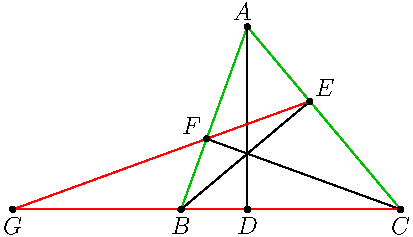
\includegraphics[scale=1]{cevian-harmonic.pdf}
	\caption{$B,C,D,G$ is a harmonic bundle.}
\end{figure}
You can prove the above lemma using just Ceva's and Menelaus's Theorem.
Note that, $AX,BY,CZ$ are concurrent hence, follows Ceva's Theorem and $E,F,G$ are collinear following Menelaus's Theorem.



\begin{lemma}[Complete Quadrilaterals Induces Harmonic Bundles] \label{lemma:com-har}
Let ABCD be 
a quadrilateral whose diagonals meet at $K$. Lines $AD$
 and $BC$ meet at $L$, and line $KL$ 
meets $AB$ and $CD$ at $M$ and $N$ . Then $(K, L; M, N)$
 is a harmonic bundle. 
\end{lemma}

\begin{figure}[h!t]
\centering
	\includegraphics[scale=1]{complete-quad-harmonic.pdf}
	\caption{$K,L,M,N$ is also a harmonic bundle.}
\end{figure}

Let $AB$ and $CD$ inersect at $P$ and $PK$ and $BC$ intersect at $Q$, then, $(Q,L,B,C)=-1$ and projecting onto the desired line through $P$ gives us the result.

Now, you can solve a problem using the results we have derived above.

\begin{example}[USA TST 2011/1]
In an acute scalene triangle $ABC$, points $D, E, 
F$ lie on sides $BC, CA, AB,$ respectively, such that $AD \perp BC, BE \perp CA, CF \perp AB$.
Altitudes $AD, BE, CF$ meet at orthocenter $H$. 
Points $P$ and $Q$ lie on segment $EF$ such that 
$AP \perp EF$ and $H Q \perp EF$ . Lines $DP$ and $QH$  intersect 
at point $R$. Compute $HQ/HR$.
\end{example}

By using \autoref{lemma:com-har},  we can derive that,  
$(A,H; AD \cap EF , D)=-1$, and projecting through $P$
 gives  $(P_{\infty}, H ; Q, R)=-1$ where $P_{\infty}$
 is the point at infinity on parallel lines $AP$ and
  $QR$ Hence, $HQ/HR=1$.

\begin{lemma}[Midpoints and Parralel Lines]
Given points $A$ and $B$, let $M$ be the
midpoint of $AB$ and $P_{\infty}$ the point at infinity of line $AB$. Then $(A, B; M, P_{\infty})$ is a harmonic bundle.
\end{lemma}

\begin{proposition}[Harmonic Quadrilateral]
$ABCD$ cyclic quadrilateral and $AC/BC = AD/BD$ then $ABCD$ is called harmonic quadrilateral.
\end{proposition}
\begin{figure}[h!t]
\centering
	\includegraphics[scale=1]{har-quad.pdf}%{harmonic-quad.png}
	\caption{Here $AXBY$ is a harmonic quadrilateral}
\end{figure}
Harmonic Quadrilateral has many nice and cute properties:
\begin{enumerate}[{\textbf (a)}]
	\ii If tangent at $B$ and $D$ meet at $T$ then, $A,C,T$ are collinear. The intersection of the diagonals ($S$) is also collinear with $A,C,T$.
	\ii $S$ and $T$ are inverse of each other with respect to $(ABCD)$.
	\ii $AC$ is an $A$-Symmedian of $DAB$ and $C$-Symmedian of $BCD$. Analogous for $BC$.
\end{enumerate}


\begin{lemma}[Right Angles and Bisectors]
Let $X,A,Y,B$ be collinear points in that order and let $C$ be any point not on this line. Then any two of the following conditions implies the third condition.
\begin{enumerate}[i]
	\ii $(A,B;X,Y)$ is a harmonic bundle.
	\ii $\angle XCY=90\dg$.
	\ii $CY$ bisects $\angle ACB$.
\end{enumerate}
\end{lemma}

\begin{figure}[h!t]
\centering
	\includegraphics[scale=1]{right-bisector.pdf}%{right-angles-bisector.png}
	\caption{$CX$ and $CY$ are external and internal angle bisectors.}
\end{figure}

\begin{lemma}[Midpoint of a Segment]
$(A,B,C,D)=-1$ and $M$ is the midpoint of $AB$, then 
\begin{itemize}
	\ii $MA^2=MB^2=MC\cdot MD$.
	\ii $DA\cdot DB = DC \cdot DM$.
\end{itemize}
\end{lemma}


\begin{theorem}[Brocard's Theorem]
Let $ABCD$ be an arbitrary cyclic quadrilateral
inscribed in a circle with center $O$, and set $P = AB \cap CD, Q = BC \cap DA, \text{and } R =
AC \cap BD.$ Then $P , Q, R$ are the poles of $QR, RP , P Q$, respectively.
In particular, $O$ is the orthocenter of triangle $PQR$.
\end{theorem}
\begin{figure}[h!t]
\centering
	\includegraphics{brocard.pdf}
	\caption{$(OAMC)$ and $(OBMD)$ are the inverses of $AC$ and $BD$ respectively.}
\end{figure}

Here we see that $R$ is the inverse of $M$. So, $O,R,M$ are collinear. 

And consequently, $PQ$ is the polar of $R$.

We shall prove that $PR$ is polar of $Q$ and $QR$ is polar of $P$.

$Q,R\in \text{ polar of }P$
So, we have from La Hire's Theorem that $P$ belongs to polar of both $Q,R$.

Then, join $Q,R$ and they intersect the circle and $AB,CD$ at four points and then doing some harmonic bundle chase gives the desired result and left as an exercise!

\section{Practice Problems}


\begin{problem}


	\begin{hint}
	\addhint{}
	\addhint{}
	\end{hint}
\end{problem}

\begin{problem}


	\begin{hint}
	\addhint{}
	\addhint{}
	\end{hint}
\end{problem}

\begin{problem}


	\begin{hint}
	\addhint{}
	\addhint{}
	\end{hint}
\end{problem}

\begin{problem}


	\begin{hint}
	\addhint{}
	\addhint{}
	\end{hint}
\end{problem}

\begin{problem}


	\begin{hint}
	\addhint{}
	\addhint{}
	\end{hint}
\end{problem}

\begin{problem}


	\begin{hint}
	\addhint{}
	\addhint{}
	\end{hint}
\end{problem}

\begin{problem}


	\begin{hint}
	\addhint{}
	\addhint{}
	\end{hint}
\end{problem}
%\section{}